\subsection{Экспериментальная апробация}

Экспериментальная апробация направлена на демонстрацию возможностей разработанного предметно-ориентированного языка.

Рассмотрим пример решения некоторой задачи с помощью DSL.
Пусть необходимо реализовать простую корзину товаров с возможностью многоразового выбора, просмотра списка выбранных товаров и их суммарной стоимости.


Полная сконструированная структура бота представлена на рисунке~\ref{f:experimentFull}.
Далее рассмотрим детально этапы построения данной структуры бота.

\clearpage

\begin{figure}[!ht]
	\centering
	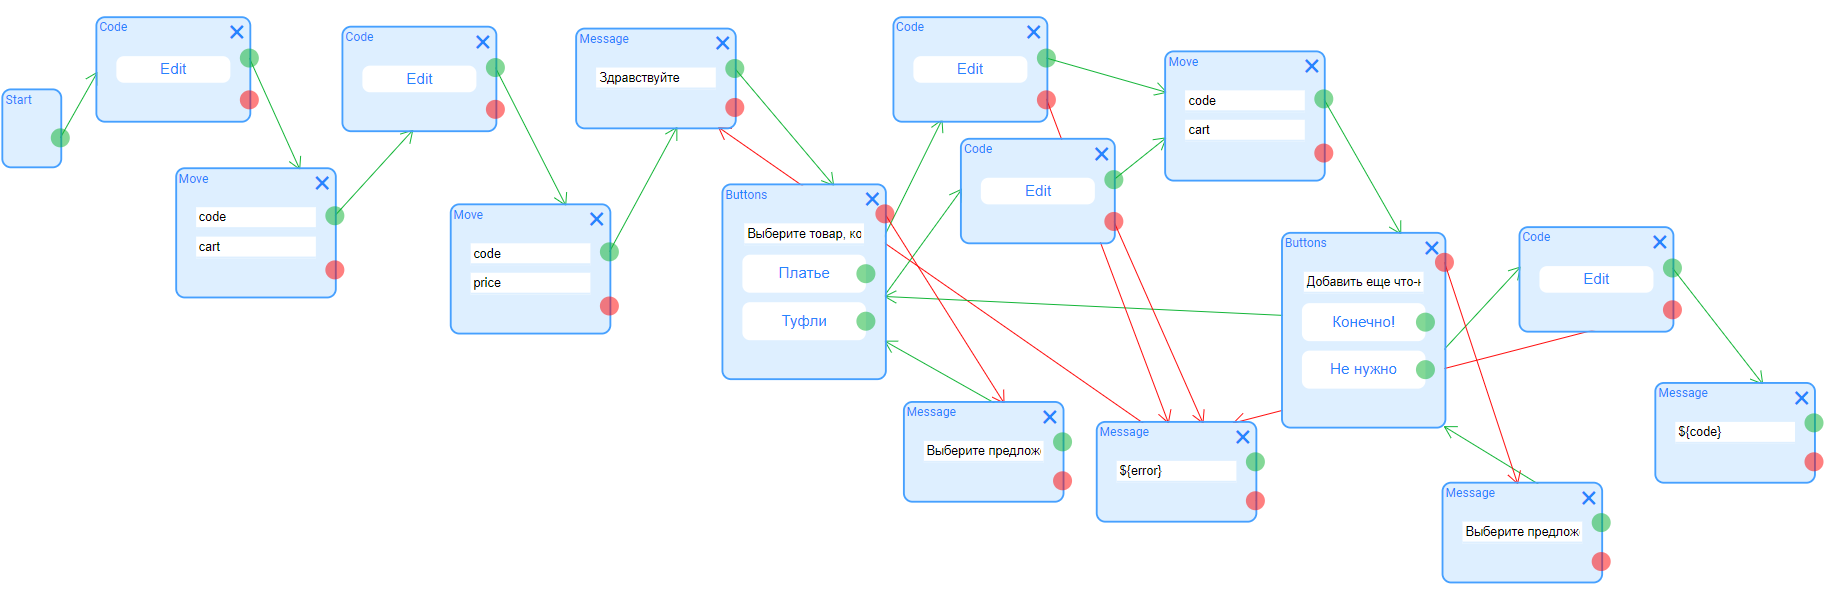
\includegraphics[width=1.0\textwidth]{testing/full.png}
	\caption{Полная компонентная структура бота}
	\label{f:experimentFull}
\end{figure}

Первоначально необходимо построить в визуальном конструкторе цепочку блоков, определяющую пользовательскую корзину и стоимость товара.
Для простоты список товаров будет состоять из двух позиций.
Цепочка, определяющая корзину и стоимость товара представлена на рисунке~\ref{f:experimentCartPrice}.
Код с объявлением стоимости единицы товара приведен на рисунке~\ref{f:experimentCodePrice}.

\begin{figure}[!ht]
	\centering
	\vspace{\toppaddingoffigure}
	\includegraphics[width=0.7\textwidth]{testing/сartPrice.png}
	\caption{Цепочка, определяющая корзину и стоимость товара}
	\label{f:experimentCartPrice}
\end{figure}

\clearpage

\begin{figure}[!ht]
	\centering
	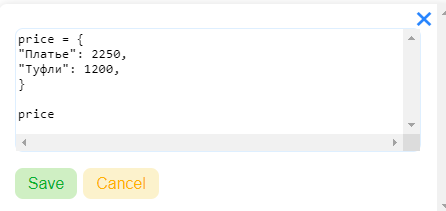
\includegraphics[width=0.6\textwidth]{testing/codePrice.png}
	\caption{Пример кода на DSL}
	\label{f:experimentCodePrice}
\end{figure}

Затем необходимо предоставить пользователю бота выбор товара. Для этого отправим сообщение с двумя кнопками,
обозначающими возможные варианты ответа. Если ответ пользователя не будет принадлежать этим возможным вариантам, запрос будет отправлен повторно.
После выбора пользователем определенного товара, увеличим количество данного товара на 1 с помощью компонента <<код>>.
Цепочка выбора товара представлена на рисунке~\ref{f:experimentSelectItem}.

\begin{figure}[!ht]
	\centering
	\vspace{\toppaddingoffigure}
	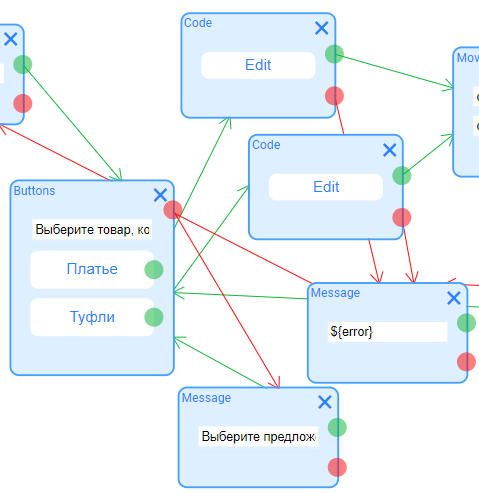
\includegraphics[width=0.45\textwidth]{testing/selectItem.png}
	\caption{Цепочка выбора товара}
	\label{f:experimentSelectItem}
\end{figure}

Код увеличения количества единиц товара в корзине при его выборе пользователем представлен на рисунке~\ref{f:expCodeAddItem}.

\clearpage

\begin{figure}[!ht]
	\centering
	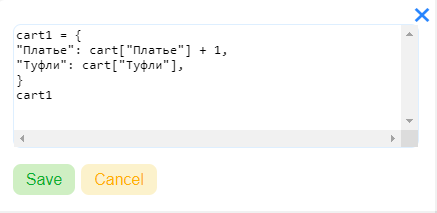
\includegraphics[width=0.6\textwidth]{testing/expCodeAddItem.png}
	\caption{Код добавления товара в корзину}
	\label{f:expCodeAddItem}
\end{figure}

После того, как пользователь выбрал товар, выполняется отправка сообщения с предложением повторного выбора товара.
В случае отказа выполняется формирование списка товаров из корзины с указанием их стоимости и общей суммы по всем позициям корзины.
Пример кода на предметно-ориентированном языке, который формирует ответ приведен на рисунке~\ref{f:endCode}.

\begin{figure}[!ht]
	\centering
	\vspace{\toppaddingoffigure}
	\begin{lstlisting}[
        language=Go,
		xleftmargin=.08\textwidth,
        xrightmargin=.08\textwidth
    ]
pprice = cart["Платье"] * price["Платье"];
tprice = cart["Туфли"] * price["Туфли"];

t = ""
if(cart["Платье"] > 0) {
	t = t + "- Платье: " + intToString(cart["Платье"]) + " ед.: " + intToString(pprice) + " р. \n"
}

if(cart["Туфли"] > 0) { 
	t = t + "- Туфли: " +  intToString(cart["Туфли"]) + " ед.: " + intToString(tprice) + " р. \n"
}

if(cart["Туфли"] == 0 && cart["Платье"] == 0) {
	t = "Корзина пуста\n"
}

s = "Ваша корзина:\n " + t + "\n Общая стоимость: " + intToString(pprice + tprice) + " р."
s
\end{lstlisting}
	\caption{Код формирования сообщения с корзиной}
	\label{f:endCode}
\end{figure}

\clearpage

Демонстрация работы запущенного Telegram бота представлена на рисунке~\ref{f:experimentDemo}.

\begin{figure}[!ht]
	\centering
	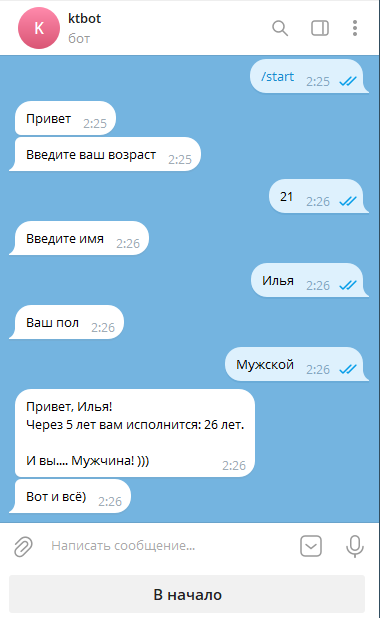
\includegraphics[width=0.6\textwidth]{testing/demo.png}
	\caption{Демонстрация работы бота}
	\label{f:experimentDemo}
\end{figure}

\section*{Вывод}
В данном разделе было проведено тестирование разработанного программного продукта.
На базе встроенной в среду выполнения Go утилиты <<go test>> были реализованы юнит-тесты, охватывающие большинство функций модуля интерпретации.

Также была выполнена экспериментальная апробация, показывающая пример расширения возможностей визуального конструктора Telegram ботов
за счет использования компонента, для запуска кода на разработанном предметно-ориентированном языке.
\clearpage

